\documentclass{scrartcl}			% defines the kind of document you want to produce

% Include different packages:
\usepackage[utf8]{inputenc}
\usepackage[T1]{fontenc}
\usepackage{lmodern}
\usepackage[english]{babel}
\usepackage{amsmath}
\usepackage{graphicx}           	% include graphics
\usepackage{caption}	
\usepackage{subcaption}	 
\usepackage{hyperref}
\usepackage{epstopdf}

\title{Neuroprothetik Exercise 2 \\ Mathematical Basics 1}
\author{ Laura Bielenberg }
\date{11. Mai 2019}


\begin{document} 					% Document begins here

\maketitle

\section{Plot slope fields and isoc lines}		% start a new section 

Plot the slope fields for t $\in [−5, 5 ]$ and V $\in [−5, 5 ] $ as well as the isoclines for $(-2, -1, 0, 1, 2) \frac{V}{s}$ for the following differential equations.

\begin{equation}
	\frac{dV}{dt} = 1 - V - t
	\label{dgl1}
\end{equation}
\begin{equation}
	\frac{dV}{dt} = \sin{t} - \frac{1}{1.5}V
	\label{dgl2}
\end{equation}

\begin{figure}[H]	
	\centering
	\begin{subfigure}[b]{\textwidth}			%start figure-environment
		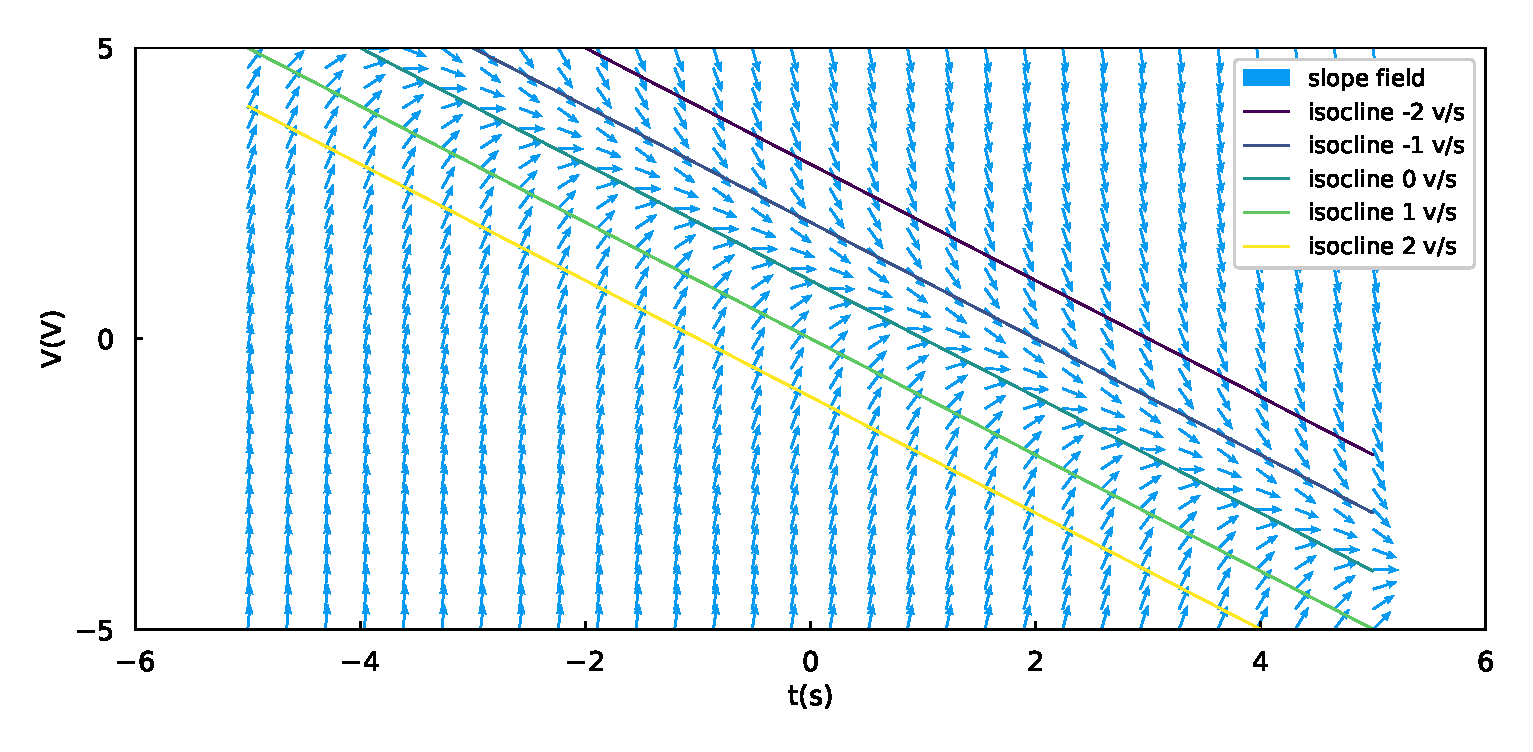
\includegraphics[width=1\linewidth]{imgs/isoclines_DGL_1.eps}
		\caption{}
		\label{fig:dgl1} %choose a label, see subsection references
	\end{subfigure}

	\begin{subfigure}[b]{\textwidth}					%start figure-environment
		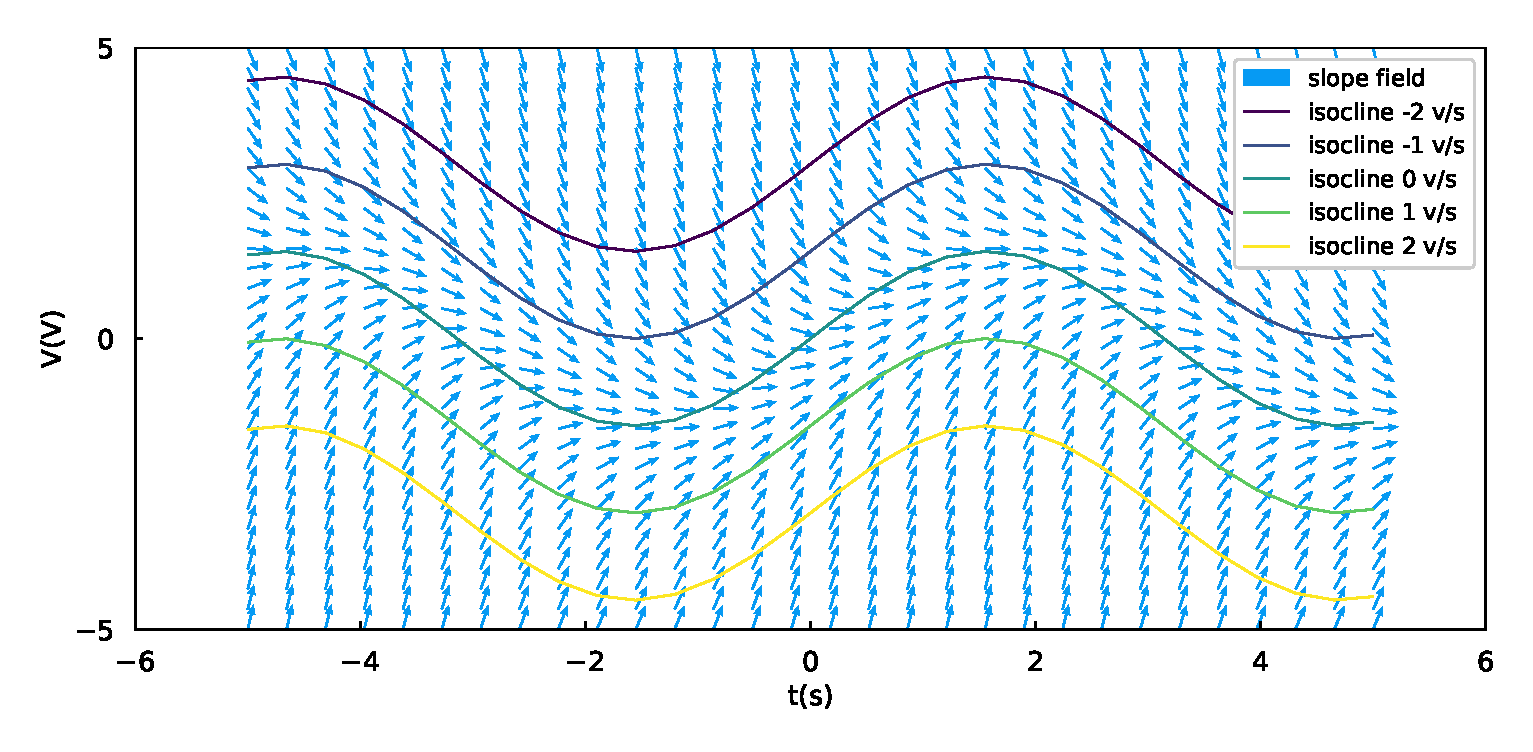
\includegraphics[width=1\linewidth]{imgs/isoclines_DGL_2.eps}
		\caption{}
		\label{fig:dgl2} %choose a label, see subsection references
	\end{subfigure}
	\caption{Plot of slope field with isoclines for differential equations. Figure \ref{fig:dgl1} for equation \ref{dgl1},  figure \ref{fig:dgl2} for equation \ref{dgl2} . }
\end{figure}

\section{Differential equations of a simple cell model}		% start a new subsection

Derive the differential equation corresponding to the integrate and fire neuron circuit, shown on the exercise sheet.

With
\begin{equation}
	I_{ex}=I_R + I_c
\end{equation}
and knowing that
\begin{equation}
	I_R = \frac{V}{R}
\end{equation}
as well as
\begin{equation}
	I_C = C * \frac{dV}{dt}
\end{equation}

the differential equation can be derived as

\begin{equation}
	\frac{dV}{dt} = \frac{I_{ex}-\frac{V}{R_{i}}}{C} = \frac{I_{max}*\sin{t}-\frac{V}{R_{i}}}{C} 
	\label{cellDGL}
\end{equation}

\subsection{Plot the slope field}
Plot the slope field for:

\begin{equation*}
	R_{i} = 1.3  \Omega, C = 0.8 F, I_{max} = 0 A
	\label{param1}
\end{equation*}
and
\begin{equation*}
	R_{i} = 1.3  \Omega, C = 0.8 F, I_{max} = 1 A.
	\label{param2}
\end{equation*}
\linespace
Add another constant term D=2 A to the current part of the differential equation and plot:

\begin{equation*}
	R_{i} = 1.3  \Omega, C = 0.8 F, I_{max} = 0 A
	\label{param3}
\end{equation*}
and
\begin{equation*}
	R_{i} = 1.3  \Omega, C = 0.8 F, I_{max} = 1 A.
	\label{param4}
\end{equation*}


\begin{figure}[H]	
	\centering
	\begin{subfigure}[b]{\textwidth}			%start figure-environment
		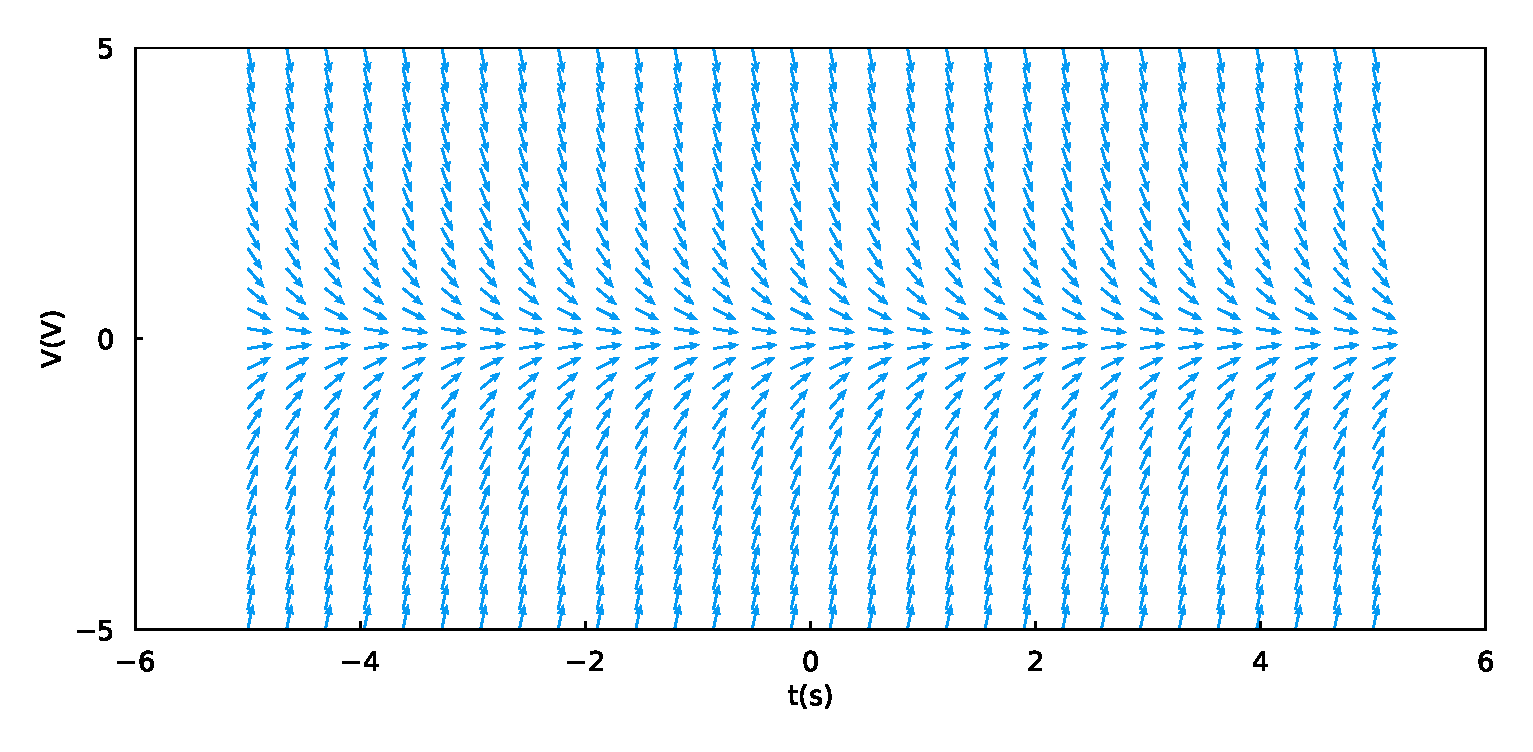
\includegraphics[width=1\linewidth]{imgs/slopes_circuitDGL_1.eps}
		\caption{}
		\label{fig:circ_dgl1} %choose a label, see subsection references
	\end{subfigure}

	\begin{subfigure}[b]{\textwidth}					%start figure-environment
		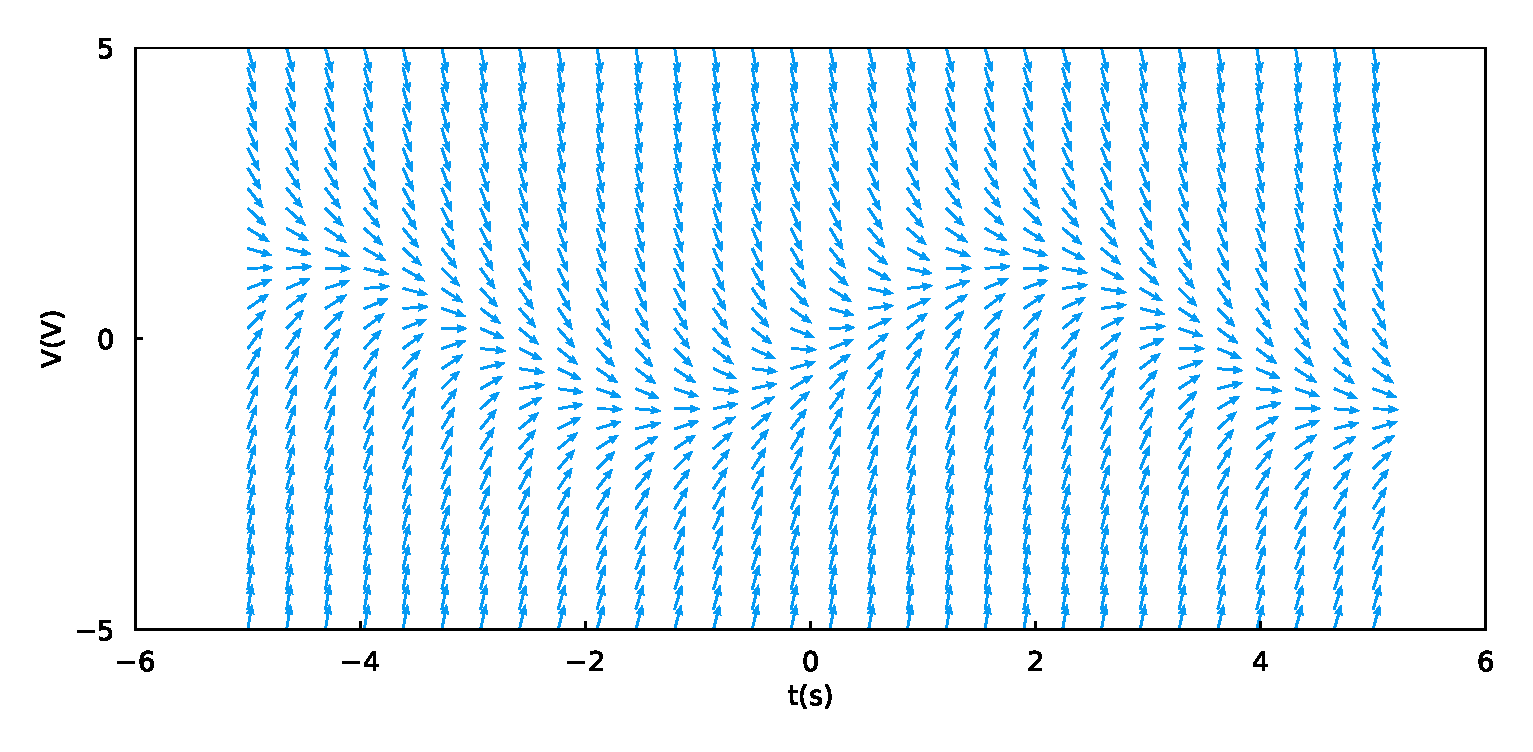
\includegraphics[width=1\linewidth]{imgs/slopes_circuitDGL_2.eps}
		\caption{}
		\label{fig:circ_dgl2} %choose a label, see subsection references
	\end{subfigure}
	\caption{Plots of slope fields for the given leaky integrate and fire neuron circuit. Figure \ref{fig:circ_dgl1} for $R_{i} = 1.3  \Omega$, $C = 0.8 F$, $I_{max} = 0 A$,  figure \ref{fig:circ_dgl2} for parameter set $R_{i} = 1.3  \Omega$, $C = 0.8 F$, $I_{max} = 1 A $.}
\end{figure}

\begin{figure}[H]	
	\centering
	\begin{subfigure}[b]{\textwidth}			%start figure-environment
		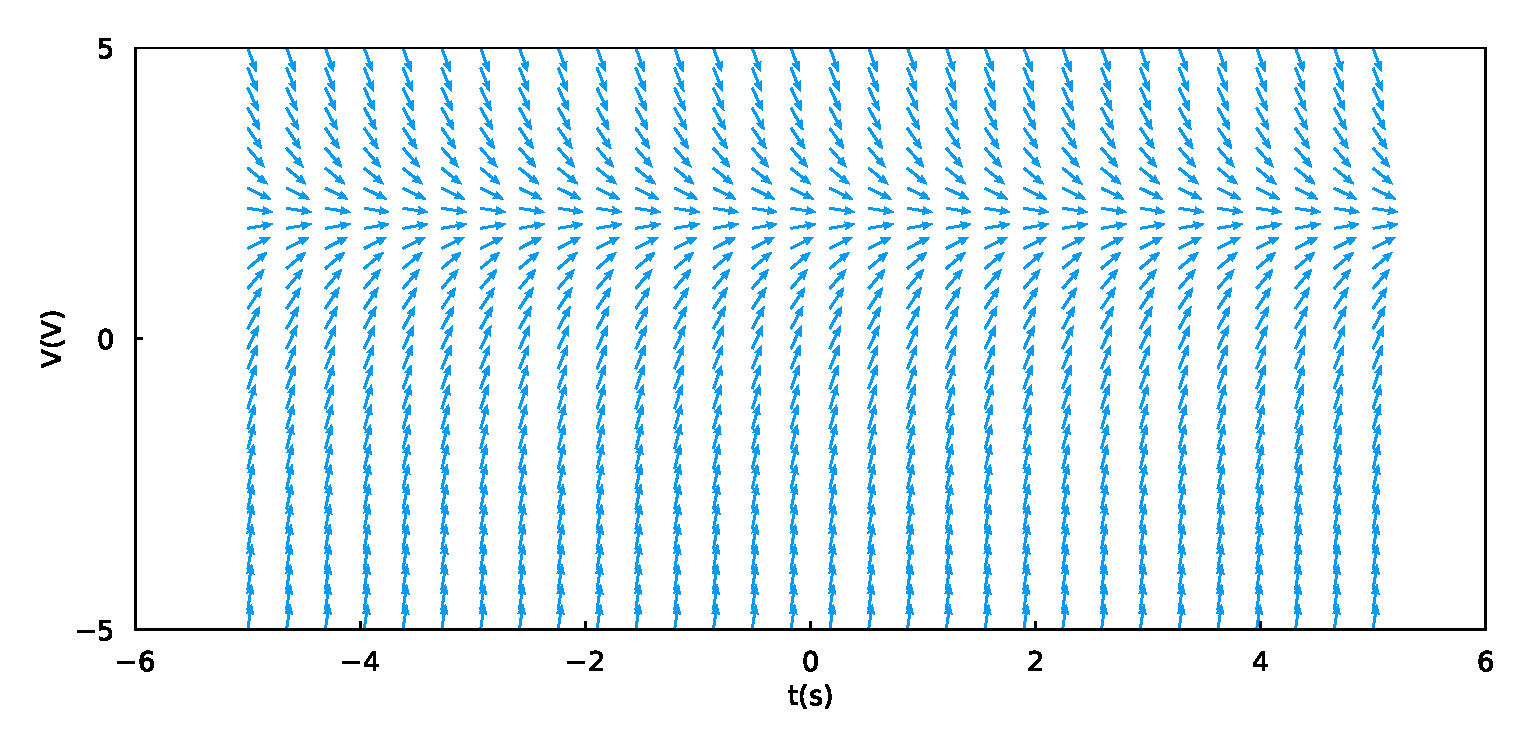
\includegraphics[width=1\linewidth]{imgs/slopes_circuitDGL_1_withConst.eps}
		\caption{}
		\label{fig:circ_dgl3} %choose a label, see subsection references
	\end{subfigure}

	\begin{subfigure}[b]{\textwidth}					%start figure-environment
		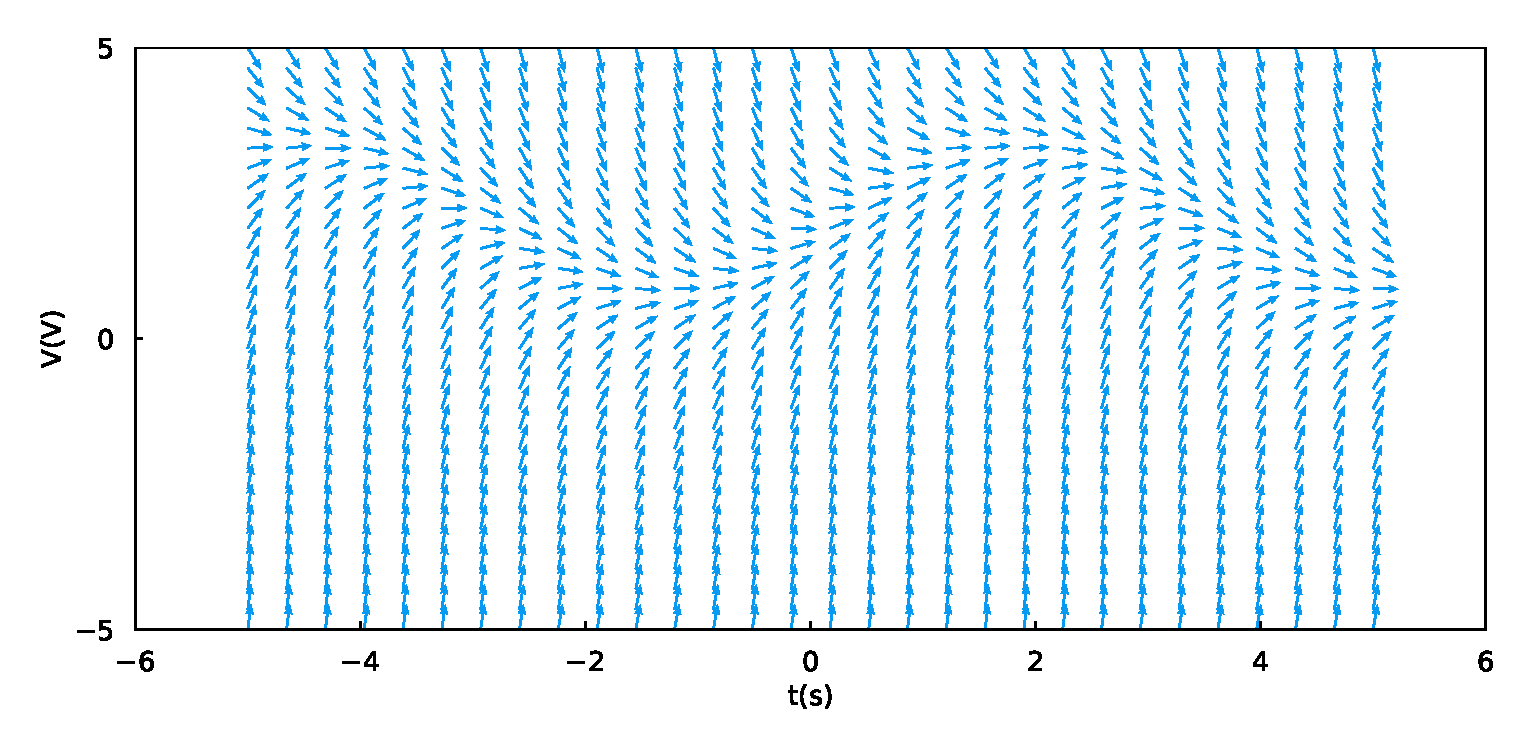
\includegraphics[width=1\linewidth]{imgs/slopes_circuitDGL_2_withConst.eps}
		\caption{}
		\label{fig:circ_dgl4} %choose a label, see subsection references
	\end{subfigure}
	\caption{Plots of slope fields for the given leaky integrate and fire neuron circuit with an additional constant D = 2. Figure \ref{fig:circ_dgl3} for $R_{i} = 1.3  \Omega$, $C = 0.8 F$, $I_{max} = 0 A$,  figure \ref{fig:circ_dgl4} for parameter set $R_{i} = 1.3  \Omega$, $C = 0.8 F$, $I_{max} = 1 A $.}
\end{figure}

\end{document}